%______________________________________________________________________________
% main.tex

\input{preamble12-screen.tex}
\hypersetup{%
    pdfauthor={Mike Pierce}%
   ,pdftitle={Math N16B Homework Five, Summer 2021}%
   ,pdfkeywords={Pierce,MathN16B,16B,N16B,Calculus,Integration,Berkeley}%
}
\usepackage{fourier}
\input{accessible-colors.tex}
\input{newcommand.tex}
\input{newenvironment.tex}
\excludecomment{solution}
\pagestyle{empty}


\begin{document}

\begin{center}
    {\Huge{Homework Five}}
    \\ \footnotesize{Analytic Geometry and Calculus}
    \\ \footnotesize{UC Berkeley Math N16B, Summer 2021}
\end{center}
\vspace{2em}

Upload your responses to the prompts marked
(\textsc{\textcolor{magenta}{Submit}})
to Gradescope before 8pm Friday; 
you will receive feedback on these.
\begin{center}
    \href{https://www.gradescope.com/courses/275664}%
    {\texttt{gradescope.com/courses/275664}}
\end{center}
The rest of the exercises you should complete at your discretion.
Note that \emph{Calculus with Applications, 11th Edition} 
has some select solutions, usually to odd-numbered exercises, in the back.


\section*{Goals this Week}

Here are some goals you should have in mind while exercising:
\begin{enumerate}
    \item 
        Extend your interpretation of a definite integral as an area 
        to higher dimensional regions. 
        Given a three-dimensional region, 
        know what double (or triple) integral calculates its volume. 
        Also given an integral, know what geometric object it's measuring.

    \item 
        Know what a \emph{differential equation} is!
        Since this is a really brief intro to the subject,  
        focus on building familiarity with the vocabulary
        Also you should know how to solve a separable ODE
        (so long as the resulting integrals aren't too tough)
        and you should be able to find the equilibrium points
        of an ODE and know what they represent if the ODE
        is modelling something.
\end{enumerate}

\newpage

\section*{Exercises}

\begin{enumerate}
    \item % Double Integrals
        I expect you to be practiced at calculating 
        iterated (double) integrals, 
        and at being able to express the area or volume of a region
        as an iterated integral. 
        The initial exercises from Chapter 9.6 of 
        \emph{Calculus with Applications, 11th Edition}
        provides you with \emph{a lot} of practice at the first
        one of these expectations, and a few for the second.
        Work through the odd-numbered exercises, or maybe every other odd exercise.
        Your choice---exercise until you feel confident.
        Also these exercises:
        \begin{center}
            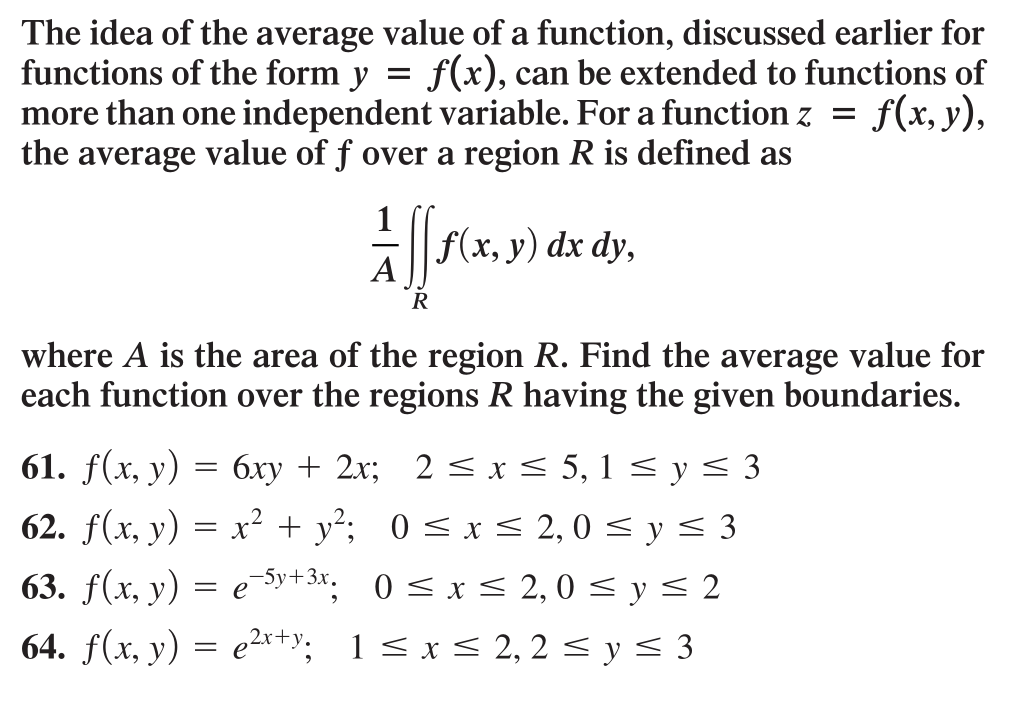
\includegraphics[width=0.96\textwidth]{screenshots/61626364.png}
        \end{center}

    \item 
        What is the volume of the region bounded in the first quadrant 
        by the plane given by the equation $(x-3) + 2(x-5) + 3(x-7) = 0$?

    \item 
        (\textsc{\textcolor{magenta}{Submit}})
        Write down an iterated integral that calculates the volume
        bounded between the surfaces
        $z + 2x^2+2y^2=36$ and $z+x^2+y^2=20$.
        Can you also set up an integral that calculates this volume
        considering the region as a solid of revolution?
        Hint: Using the disk method you'll need 
        the difference of two integrals, one corresponding to a volume
        you want to subtract from the other.
        Which one of these looks easiest to evaluate?

    \item 
        Estimate the volume of the space in the first quadrant 
        bound between the curves
        \begin{equation*}
            xyz=1 \qquad\text{and}\qquad x+y+z = 11
        \end{equation*}
        I say ``estimate'' because find this exact volume is tough, 
        but if you set it up as an integral $\iint_R f \,\mathrm{d}R$
        for some region $R$ in the $(x,y)$-plane, 
        that $R$ is \emph{almost} a triangle,
        which allows you to get an easy estimate. 

    \item 
        What is the volume of the dome-shaped region over the point $(0,0,0)$
        trapped between the graph of $f(x,y) = \cos(\sqrt{x^2+y^2})$
        and the $(x,y)$-plane?
        Also, write down an integral that calculates
        this volume considering the region as a solid of revolution.

    \item 
        What is the volume of a region bound by the three cylinders,
        each of radius one, and each centered along one of the $x$-,
        $y$-, and $z$-axis?
        Is this bound region a sphere?

    \item 
        What is the volume of the region bounded by
        \begin{equation*}
            x^2+y^2=z^2
            \qquad
            \text{and}
            \qquad
            x+y=2z+1
        \end{equation*}

    \item 
        You have a bowl full of water. 
        The surface of the bowl has the same shape as the graph 
        of the function $f(x,y) = x^4+y^4$ for $0 \leq z \leq 4$.
        You tilt the bowl $30^\circ$, spilling out some of the water.
        What is the volume of the remaining water?

    \item
        %%% SHELL
        Consider a grain silo with a base that is a perfect circle
        $200$ meters across. The walls of the silo stretch skyward $900$ meters
        before meeting with a parabolic roof.
        The very tip of the parabolic roof, 
        the highest point on the silo, is $1000$ meters above the ground. 
        Write down a double or triple integral
        that calculates the volume of this silo.

        Write down an integral
        that calculates the volume of this silo
        considered as a solid of revolution.

    \item % Intro to ODEs, Separable and Equilibrium Points
        When you see an ODE, you should certainly immediately check
        if it's a separable ODE. I expect that you should be able 
        to separate a separable ODE, write it as $M(y) \dy = N(x)\dx$
        for some function $M$ and $N$.
        Additionally you should be able to identify equilibrium points
        of an ODE and talk about their stability.
        The initial exercises from Chapter 10.1 of 
        \emph{Calculus with Applications, 11th Edition}
        will help you develop these two skills.
        Work through those exercises until you feel confident.

    \item
        Verify that each of the following is a solution 
        to the given differential equation.
        \begin{enumerate}
            \item Verify that $p(t)=3\ex^{kt}$ is a solution to $p'=kp$.
            \item Verify that $y=2t^3$ is a solution to $3yy'''=y'y''$.
            \item Verify that $y(t)=\cos(2t)$ is a solution to $yy'+\sin(4t)=0$.
            \item Verify that $y(t)=\cos(2t)$ is also a solution to 
              $yy''+4=(y')^2$.
        \end{enumerate}

    \newpage

    \item
        Give me an example of a single-variable function
        such that the product of that function with its derivative 
        is equal to two.

    \item 
        Solve these differential equations.
        Notice that I'm not providing any initial conditions,
        so I'm asking for the \emph{general} solution to each of these.
        \begin{tasks}(2)
            \task $y\dot{y} + y^2 = 3ty\dot{y}+1$
            \task $y'\cot^2(x) + \tan(y) = 0$
            \task $xy' - 27y' = 3(y-9)$
            \task $(ty)^2+2y^2 + \dot{y} = 0$
            \task $2\cos(t) = 3t^2-y'$
            \task $y'-6y = 4$
            \task $xy' - 2y' = 2(y-4)$ (\textsc{\textcolor{magenta}{Submit}})
        \end{tasks}

    \item 
        Solve these differential equations.
        Notice that I'm providing you with initial conditions 
        for these differential equations, so these are examples
        of \emph{initial value problems}, and I'm asking for a
        \emph{particular} solution to each of these.
        \begin{tasks}(1)
            \task $\frac{1}{t}\sec^2(y)\frac{\mathrm{d}y}{\mathrm{d}t} = 1$ 
            where $y(0)=1$
            \task $\ex^t - yy' = 0$ where $y(0) = 3$
            \task $y'' =  x^2 + 3$ where $y=-4$ and $y'=2$ when $x=0$.
        \end{tasks}

    \item 
        (\textsc{\textcolor{magenta}{Submit}})
        Some wildlife conservationists want to reintroduce 
        flamingos to an uninhabited region where flamingos once thrived
        before being wiped out from excessive hunting.
        After introducing an initial population of flamingos to the region,
        the conservationists suspect that the differential equation
        \begin{equation*}
            \frac{\mathrm{d}P}{\mathrm{d}t} 
            = -\frac{1}{2}\left(P^3-4P^2+3P\right)
        \end{equation*}
        will be an accurate model for the population of flamingos over time, 
        where $P(t)$ is measured in thousands of flamingos 
        after $t$ years of introducing the flamingos.
        What is the \emph{carrying capacity} of the population
        according to this differential equation?
        According to the model, how large does the initial population need to be
        to ensure that the population survives?

    \item 
        Some question about models:
        \begin{center}
            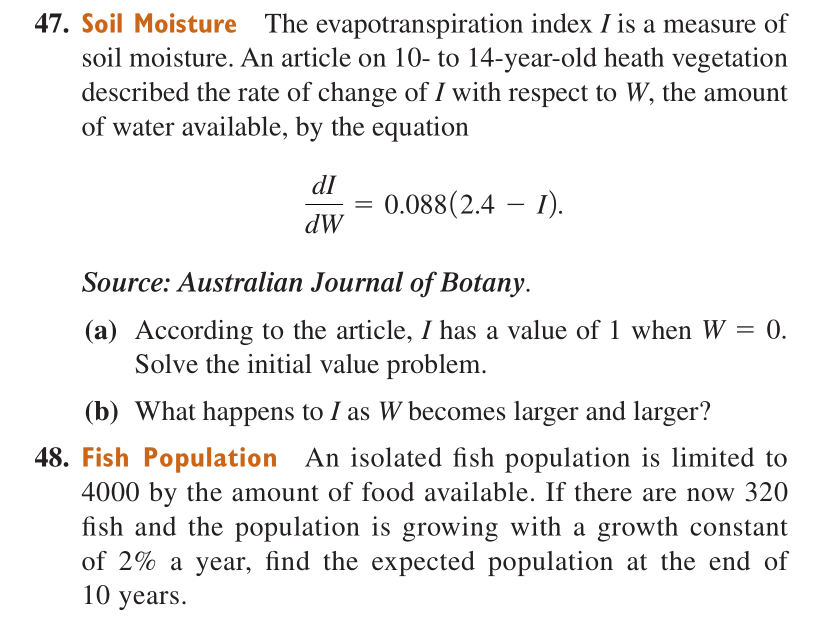
\includegraphics[width=0.96\textwidth]{screenshots/4748.png}
        \end{center}

    \item 
        \begin{center}
            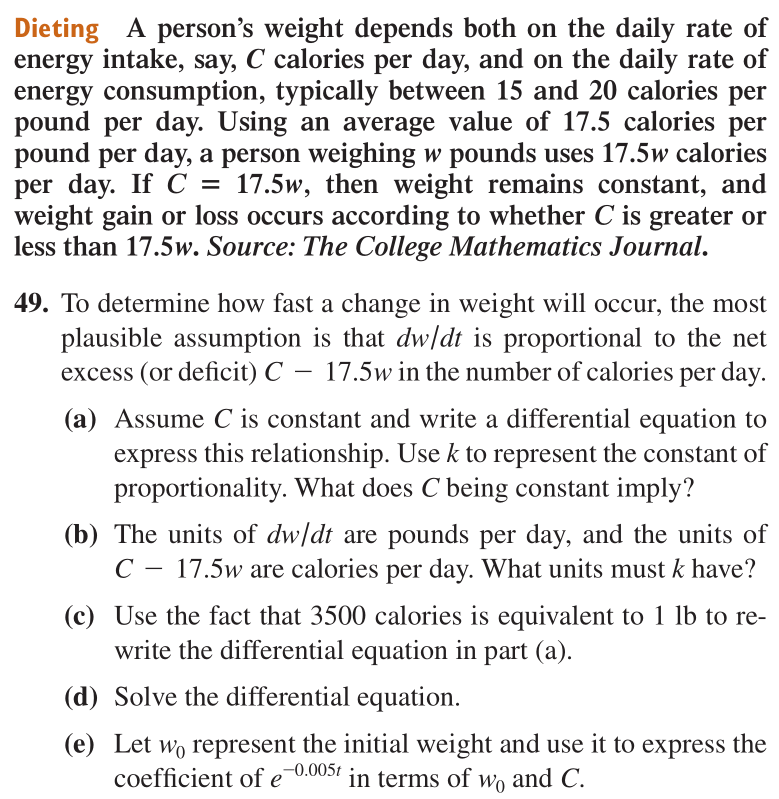
\includegraphics[width=0.96\textwidth]{screenshots/49.png}
        \end{center}

    \item 
        (\textsc{Recreation})
        Three friends Anita, Becca, and Charleston 
        are challenged to a game by the Game Maestro.
        The Game Maestro places two colored dots 
        on each of the friends' foreheads
        and tells the friends that each dot is either blue or yellow,
        but neither color is used more than four times.
        He then places the three friends in a circle so that each of them
        can see the dots on their friends' foreheads, but not on their own.
        Then the game goes like this:
        The Maestro will ask the friends in turn, 
        first Anita, then Becca, then Charleston, then Anita again, 
        then Becca again, and so on, 
        if they know the colors of the dots on their foreheads.
        If someone responds ``no,'' the Maestro asks the next person.
        If someone responds ``yes'' and is right, the friends win!
        Whereas if someone responds ``yes'' and is wrong, 
        all three friends will be banished to the shadow realm.

        The friends were given no time to strategize, 
        but they begin playing. Their responses in turn are
        \begin{center}
            no 
            \hspace{2ex}
            no 
            \hspace{2ex}
            no 
            \hspace{2ex}
            no 
            \hspace{2ex}
            yes
        \end{center}
        and the three friends win! 
        Whare are the colors of the dots on Becca's forehead?

\end{enumerate}

\end{document}

